\label{sec:conclusions}
\par This document has presented a measurement of $\nu_e$ events in the Booster Neutrino Beamline with the MicroBooNE experiment. The analysis leverages sophisticated reconstruction tools which take advantage of scintillation light and detailed calorimetric and spatial information from MicroBooNE's TPC in order to produce a kinematically agnostic measurement of electron neutrinos with any number of final-state protons and no final state pions. The analysis, while aiming to perform a robust measurement across a broad energy range, tailors many of its selection and analysis-level choices to be sensitive to low-energy electron neutrinos, where the complex event topology and high rate of $\nu_{\mu}$ CC and NC backgrounds make the analysis challenging. At the same time, the focus on the sub-GeV energy region allows for analysis sensitivity to anomalies similar to that observed by the MiniBooNE experiment. The analysis reaches a median sensitivity for discovery of a MiniBooNE-like $\nu_e$ signal of $2.6\sigma$ with full statistical, flux, genie, and detector systematics, after the $\nu_{\mu}$ constraint. The sensitivity of the analysis is summarized in figure~\ref{fig:sensitivity_bdt_loose_const:conclusions} and table~\ref{tab:sensitivity}.

\begin{figure}[H]
    \begin{center}
    \begin{subfigure}{0.55\textwidth}
    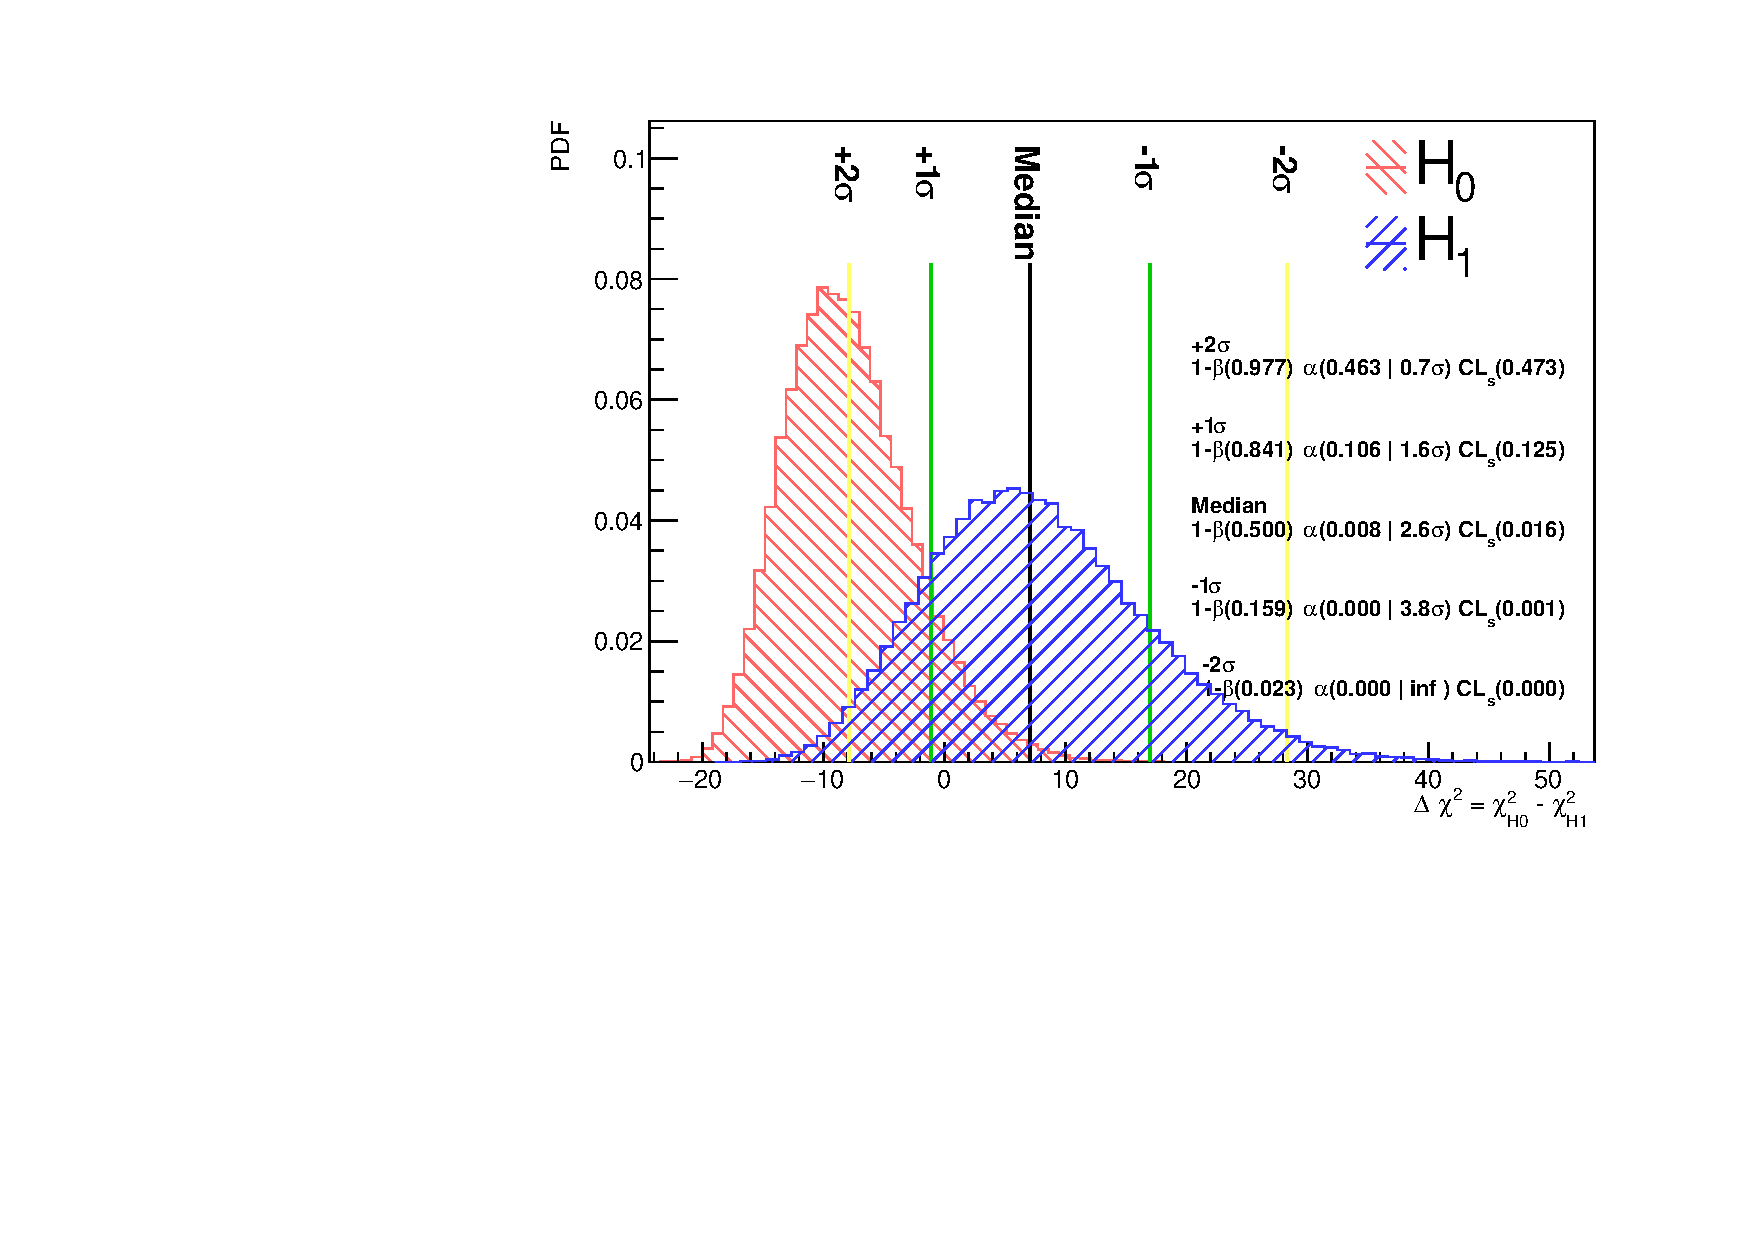
\includegraphics[width=1.00\textwidth]{Sensitivity/BDT_higheff/SBNfit_Cls_nue_1e0p_numu_reco_e_H1_newBDT_higheff_noCCMEC_constrained_detsys.pdf}
    %\caption{Loose BDT selection}
    \end{subfigure}
    \caption{\label{fig:sensitivity_bdt_loose_const:conclusions}Final discovery sensitivity to the LEE unfolded signal of the \npsel selection with the constrained systematics.}
    \end{center}
\end{figure}

\begin{table}[H]
\centering
\setlength{\tabcolsep}{10pt}
\renewcommand{\arraystretch}{1.25}
 \begin{tabular}{| c | c | c | m{2.3 cm} | c | c | c |} 
 \hline
 POT & LEE events & \nue events & scenario & stat. $\sigma$  & stat+syst. $\sigma$ & constrained $\sigma$ \\
 \hline
\multirow{2}{*}{$6.95E20$} &  \multirow{2}{*}{14.97} & \multirow{2}{*}{74.97} & ruling out SM if LEE is true & $2.5$ & $1.9$ & $2.3$ \\
 &  &  & ruling out LEE if SM is true & $2.2$ & $1.9$ & $2.2$ \\
\multirow{2}{*}{$12.5E20$} & \multirow{2}{*}{26.91} & \multirow{2}{*}{134.85} & ruling out SM if LEE is true & $3.3$ & $2.3$ & $3.0$ \\
 &  &  & ruling out LEE if SM is true &$3.0$ & $2.5$ & $2.9$ \\
 \hline
 \end{tabular}
 \caption{\label{tab:sensitivity}Expected sensitivity for run 1-3 data and the run 1-5 data. Event counts are scaled to $6.95E20$ POT and 12.5E20 and include both \npsel and \zpsel LEE signal events.}
\end{table}


\begin{comment}
\begin{table}[H]
\centering
\setlength{\tabcolsep}{10pt}
\renewcommand{\arraystretch}{1.25}
 \begin{tabular}{| c | c | c | c | c | c |} 
 \hline
 channel & LEE events & \nue events & stat. $\sigma$  & stat+syst. $\sigma$ & constrained $\sigma$ \\
 \hline
box-cut \npsel & 10.6 & 51.6 & $2.7$ & $2.3$ & $2.5$ \\
BDT-based \npsel & 14.1 & 74.7 & $2.8$ & $2.3$ & $2.6$ \\
 \hline
 \end{tabular}
 \caption{\label{tab:sensitivity}Expected sensitivity for the Box-Cut and BDT selections of the analysis. Event counts are scaled to $10.1E20$ POT.}
\end{table}
\end{comment}

\par The analysis, as designed and presented, has demonstrated to be robust against detector mis-modeling and time-dependence in MicroBooNE's dataset. The review of this work by the entire MicroBooNE collaboration, if successful, should result in a box-opening of the $6.96e20$ POT collected through Runs 1, 2, and 3. After the processing of data from Runs 4 and 5, and the implementation of specific time-dependent calibrations for such datasets, the analysis will be ready to be processed over the full MicroBooNE dataset.


\begin{comment}

%\subsection{Remaining Steps in the Analysis}
\subsection{Remaining Steps in the Analysis}
\label{sec:conclusions:future}
\par This Tech-Note describes the analysis from beginning to end, and it aims to provide the necessary information with which to evaluate the robustness and readiness of the analysis in preparation for the final box-opening. As sidebands in \numu and \nue channels are opened, detailed data-mc comparisons from those studies will be reported in this note as additional chapters. 
\par Finally, it is worth mentioning that there are several remaining steps to be completed by the analysis. 
We list them below. Feedback from collaborators on these items is welcome. 
\begin{enumerate}
    \item \textbf{detector systematics for \zpsel selection and backgrounds} As discussed in sec.~\ref{sec:detsys:selections} the statistics available in MC samples are not sufficient to fully evaluate detector systematics for the \zpsel selection and on background samples generally. Additional work is needed to validate the 20\% flat uncertainties used for these categories of events, and updating them if necessary. 
    \item \textbf{symmetric detector systematics} Detector variation samples are to be considered corrections of the CV based on measured data-mc differences. As such, they are inherently one-sided. In SBNFit however, these errors are treated as Gaussian and two-sided. Updates in the sensitivity calculation framework to account for this effect need to be completed, or the impact of the current approximation needs to be better understood.
    \item \textbf{Sensitivity calculation} The \zpsel is included in the sensitivity through the constraint of various systematics but not in the $\Delta\chi^2$ calculation. The final sensitivity will include in the $\Delta\chi^2$ the \zpsel selection.
    \item \textbf{CCMEC systematics} The CCMEC unisim variation leads to significant uncertainty (of order 400\% in the lowest energy bin, and 100\% at higher energies) as illustrated in figure~\ref{fig:geniesystvars}. While the analysis is able to constrain these uncertainties through the \numu constraint, the true uncertainty associated with this variable needs to be better understood. If the expected variation is comparable to what currently seen, this generator uncertainty needs further scrutiny.
    \item \textbf{$\pi^0$ Modeling} Background rates for $\pi^0$ interactions as included in the sensitivity and stacked \nue distributions shown do not yet take into account the scaling of $\pi^0$ production rate of 0.76 needed to obtain agreement between data and simulation and described in sec.~\ref{sec:sideband:pi0}. This means that the $\pi^0$ rate currently used to produce final results is over-estimated. The $\pi^0$ contribution to backgrounds will be updated based on the findings observed.
    \item \textbf{Low-energy xsec modeling} The \numu constraint is particularly valuable in constraining modeling uncertainties in the rate of low energy \nue interactions. Special emphasis is being put on making sure the significant cross-section uncertainties at low energy are well constrained by the \numu selection described in sec.~\ref{sec:numuselection}. These studies are ongoing and regularly presented at MicroBooNE Genie-tune meetings.
    \item \textbf{one vs. two-sided quoted sensitivity} The sensitivity is quoted in unity of ``sigma'' ($\sigma$). This quantity is calculated by converting the p-value obtained from the test statistic distribution can be transformed to the one of a Gaussian using a one sided or a two sided test. In high energy physics the one sided value is used by convention. In this work, the SBNfit results uses a two-sided conversion. It is important to address the ambiguity caused by the choice of convention before releasing results to the community.
    \item \textbf{validate current studies with 100 universes and update / increase if needed.} For technical reasons, the analysis as presented in this note, relies on 100 flux and genie universes to compute systematic uncertainties. Increasing the number of universes used for a final result should be explored.
    \item \textbf{merging of R1+R2+R3} Currently the expected sensitivity in the analysis is obtained taking R1,R2, and R3 overlay MC samples, summed together, and scaled to the full POT. Proper POT scaling according to each run, while a minor update to the analysis in terms of performance, needs to be implemented.
    \item \textbf{GEANT4 re-interaction uncertainties} While not expected to be significant, these uncertainties must be incorporated in the analysis once available for processing.
    \item \textbf{$\Delta \chi^{2}$ Calculation} The calculation of the $\Delta \chi^{2}$ distribution in the sensitivity calculation is currently performed using the covariance matrix on the null hypothesis as we do not associate any errors on the LEE unfolded signal model. The construction of the covariance matrix that goes into the $\Delta \chi^{2}$ calculation still need to be scrutinized for both hypotheses. 
    \item \textbf{Exclusion Sensitivity} In addition to discovery sensitivities, the analysis must evaluate and validate the $\Delta \chi^{2}$ test to exclude the LEE hypothesis.
\end{enumerate}{}

\end{comment}

\begin{comment}
\begin{enumerate}
    \item \textbf{MC Statistics} Larger MC statistics for specific background categories are needed to be able to better train the \npsel BDT as well as obtain a more accurate estimation of expected backgrounds from different background neutrino categories. Initial samples for specific background categories have been generated (with $\times2-8$ the stats from the default BNB simulation, depending on the sample). It is expected that these will be included in the analysis by the Feb. 2020 collaboration meeting. %\textcolor{green}{Giuseppe}
    \item \textbf{BDT Selection and Sensitivity} Once larger MC samples are avilable, we plan to finalize the BDT based selections and produce updated sensitivities. This work will be performed by the February meeting. %\textcolor{green}{Giuseppe, David, Sophie, Wouter}
    \item \textbf{Common Optical Filter} An optical-based filter rejects MicroBooNE data with less than 20 photo-electrons of prompt light activity in the beam spill. This cut is not applied in simulation. Information for whether simulated events pass this cut is now stored in our analysis NTuples and this cut will be fully incorporated by the Feb. collaboration meeting. This cut has minimal effect on Run 1 analyses (where the \texttt{SliceID} provides a more aggressive cut) but becomes relevant in Run 3 data/simulation comparisons. %\textcolor{green}{David}
    \item \textbf{Charge re-calibration} A discrepancy in d$E$/d$x$ measured for both tracks and showers indicates a few-percent mis-calibration. In order to further improve data-simulation agreement. This re-calibration, outlined in DocDB 26438 is being implemented in the analysis code and should be incorporated in the analysis by the February collaboration meeting. %\textcolor{green}{Nicolo, David}
    \item \textbf{LLR-PID $e-\gamma$ Separation} The analysis team is exploring applying a log-likelihood based PID for $e-\gamma$ separation, in a similar way to that developed for tracks (see~\ref{subsec:loglikelihoodpid}). The goal is to further improve the rejection power for photons in the $\nu_e$ selections. Preliminary work on this will be reported at the February collaboration meeting but possibly will not be integrated in the full analysis until later in the spring.%\textcolor{green}{Nicolo}
    \item \textbf{Detector Systematics} Not all samples are currently available. Those available have been processed, and a preliminary study of their impact on reconstructed variables and efficiencies was presented. Their full inclusion in the sensitivity estimation is however dependent on certain development needed in SBNFit. We expect to also be able to fully include detector systematic uncertainties by February meeting.%\textcolor{green}{David, Maya}
    \item \textbf{$\nu_{\mu}$ Constraint Implementation} An upadted $\nu_{\mu}$ selection focused on reconstructing low-energy $\nu_{\mu}$ interactions was developed for this note. This selection, presented in section~\ref{ssec:NuMUCCsel:constr}, is now being used to test and validate the constraint procedu. Result of this work will be ready by the February collaboration meeting.%\textcolor{green}{Maya, Ryan}
    \item \textbf{Additional Sideband Constraints} The analysis is well positioned to use the \texttt{SliceID} (sec.~\ref{sec:sliceID}) and inclusive $\nu_{\mu}$ selection (sec.~\ref{ssec:NuMUCCsel:INC}) to perform exclusive final-state measurements with the purpose of constraining particular detector, flux, or neutrino interaction uncertainties. Pursuing these additional sideband measurements will be guided by concerns over the dominant sources of systematic uncertainties identified as the analysis is reviewed. These efforts are likely to occur in the time interval between the Feb. and April collaboration meetings. A first candidate for such a constraint comes from the $\pi^0$ sideband which will be used to control $\pi^0$ production uncertainties.
    \item \textbf{Box Opening Strategy} The contents of this note show generally good data-simulation agreement. As the collaboration moves towards opening the full $10.1E20$ POT for the analysis, this team would like to be able to open two intermediate datasets. First, we ask to be able to explore data-mc agreement on a $5E19$ POT dataset of Run 3 to validate that the changes in detector state have not led to discrepancies in the neutrino analysis. Second, we request to be able to open a significant fraction of the Run 3 dataset filtered through the $\nu_e$ inclusive selection (sec.~\ref{sec:nueselection:inclusive}). In order to preserve blindness to the MB-$\nu_e$ LEE model, we are considering opening up only events which pass a certain energy cut. We believe this cross-check is necessary as it helps validate modeling of $\nu_e$ interactions at higher energies before investigating a potential excess at lower energies.
    %\item MCS fitter for better efficiency for low-energy showers.
\end{enumerate}{}
\end{comment}{}